\documentclass[12pt, letterpaper, twoside]{article}
\usepackage[utf8]{inputenc}
\usepackage{dirtytalk}
\usepackage{graphicx}
\usepackage{amssymb}
\usepackage[backend=biber,style=numeric, natbib=true, sorting=none, maxbibnames=13, url=false]{biblatex}
\addbibresource{ge-refs.bib}


	
\title{Linking amino acid sequences to sources and fates of organic matter in aquatic systems}
\author{Megan Duffy}
\date{April 21, 2020}

\begin{document}
	
	\begin{titlepage}
		
		\maketitle
		\begin{center}
			A description of proposed Ph.D. dissertation research \\
			\bigskip
			\bigskip
			Supervisory committee \\
			\bigskip
			Rick Keil (chair) 
			
			Jeff Richey 
			
			Gabrielle Rocap 
			
			Anitra Ingalls 
			
			Sarah Stroup (GSR)
		\end{center}
		
	\end{titlepage}
	

\newpage

\tableofcontents{}

\newpage

\section*{Overview}

Proteins enact life’s intent: directed by genes and informed by the environment. These macromolecules are the engines that power the cells of all biological entities on Earth – from viruses and bacteria to humans and blue whales – proteins serve a vast range of metabolic, transport, communication, and structural purposes. Life, in turn, along with geological and chemical drivers, modulates the planetary cycles of carbon, oxygen, and nitrogen: at the foundation of photosynthetic fixation of atmospheric CO\textsubscript{2} into organic carbon is a suite of proteins, enzymes shuttling electrons, transforming energy from the sun into stored fuel. 

Through unlocking the information stored in peptide and protein sequences, we learn the biological origins and functions of cells within a community. For organic geochemists, there is useful information here as well: their biological function aside, proteins make up a large proportion of organic carbon and nitrogen in aquatic systems. Thus, the cycling and degradation dynamic of proteins is of great importance when thinking about global organic carbon preservation and sequestration. In applying the recent developed tools of systems biologists, we can begin to disentangle the origins and organic matter, as well as the metabolic means of its breakdown.

\textbf{My proposed Ph.D. research addresses the cycling of proteins and protein-derived organic matter in both laboratory settings and environmental systems.} Chapter 1 of my Ph.D., my M.S. project, describes the usefulness of integrating a different kind of peptide sequencing, \textit{de novo} sequencing, into the traditional environmental proteomics workflow in order to access degraded and unanticipated sequences. This is described in \say{Protein cycling in the eastern tropical North Pacific oxygen deficient zone: a \textit{de novo}-assisted peptidomic approach}, [Duffy et al., \textit{in review}]. The three following projects utilize this technique to ask questions about proteins and peptide cycling in complex environmental systems. 

Chapter 2 uses the \textit{de novo}-assisted peptidomic technique to follow the peptides of a diatom through a simulated bloom and subsequent degradation by a natural microbial community. Chapter 3 is a peptidomic-based comparison of organic matter across seasons, stations (on and offshore) and sinking class of marine organic matter in an ODZ. Chapter 4 moves out of the purely marine realm and bridges the span between terrestrial and marine systems in the Amazon River-Atlantic continuum, probing how organic matter travels from land to sea, and how microbes alter its reactivity and character.

\newpage

\section{Proposed work}

\subsection{{Chapter 1: De novo}-assisted peptidomics helps in the study of marine carbon flux and protein degradation}

Developments in high resolution mass spectrometry and computing have facilitated metaproteomic investigations of proteins in suspended \cite{dong_characterization_2010, bridoux_suspended_2015, bergauer_organic_2017} and sinking \cite{moore_identifying_2012} organic matter. These powerful metaproteomic tools could help resolve questions about protein and peptide degradation in the ocean, but they are currently limited in that they are designed to identify proteins from living biomass, often reliant on genomic or transcriptomic information derived from the same (or very similar) sample.  

Current metaproteomic workflows adhere to a bottom-up proteomic approach, relying on peptide-spectrum matching through database searching \cite{saito_progress_2019}. In this regime, proteins from the extracted environmental sample are proteolytically digested with an enzyme (often trypsin) that site-specifically cleaves proteins at known amino acid residues to generate a complex mixture of peptides. These resulting peptides are then separated by liquid chromatography and analyzed by high resolution mass spectrometry (LC-HRMS). Mass spectra from these observed peptides (precursor mass spectra, or MS) along with their fragmentation product spectra (MS\textsuperscript{2}) are then compared with theoretical spectra generated from an \textit{in silico} digestion of protein sequences within a database, a process referred to as peptide-spectrum matching. Typically, these protein sequence databases are derived either from complementary metagenomic or metatranscriptomic analyses, a compilation of annotated reference proteomes of taxa thought likely to be represented in the sample, or a combination of these two. This approach has limitations given a) the taxonomically diverse and uncharacterized nature of environmental samples, and b), the fact that proteins often deviate from gene product predictions due to alternative splicing, mutations, polymorphisms, or post-translational modifications (PTM) as a result of that protein’s intended biochemical function or through degradative processes \cite{kim_methionine_2014}. Indeed, it is typical that fewer than half of all tandem mass spectra acquired in shotgun proteomics experiments are successfully matched to a peptide from a database \cite{chick_mass-tolerant_2015}. 

\textit{De novo} sequencing is a database-independent tool that uses the same tandem mass spectral information as a peptide-spectrum matching analysis. Rather than comparing peptides to a protein database, first principles-based algorithms are used to establish sequences directly. Several styles of \textit{de novo} sequencing algorithms exist, but all use the \textit{de novo} respective mass differences between fragment ion peaks to piece back together the original MS peptide ion amino acid sequence.  Historically the original method of protein sequencing, \textit{de novo} is now mainly used in antibody peptide sequencing (i.e., only when a database-derived sequence is unavailable). This is because \textit{de novo} sequencing is generally less accurate than database searching, often because of insufficient mass accuracy \cite{muth_navigating_2015} or uneven fragmentation patterns in tandem mass spectrometry \cite{lu_algorithms_2004}. But analogous to antibodies peptides, degraded peptides are inherent unknowns in the environment. They are difficult to predict or make a database entry for, but surely are present and highly relevant to organic matter cycling. 

\subsubsection{Benchmark: \textit{Prochlorococcus marinus} culture}

Due to its database independence, \textit{de novo} sequencing has exciting potentials for complementing the traditional database-driven approach to environmental peptidomic and proteomic studies. The number of studies using any kind of \textit{de novo} peptide sequencing in environmental samples is small \cite{muth_evaluating_nodate}, but will likely grow with as mass spectrometer resolution and scanning power increase. As such, it is critical to evaluate the accuracy of this tool in a well-characterized system. As a benchmark study, I compared the sequencing performance of a well-established \textit{de novo} algorithm against a traditional database search on a \textit{Prochlorococcus marinus} culture protein dataset. \textit{P. marinus}, a ubiquitous free-living marine cyanobacterium found throughout the world’s oceans \cite{chisholm_novel_1988}, was an advantageous marine microbe for this assessment given its small and relatively well-characterized proteomes \cite{paul_distinct_2010}.

\begin{figure}
	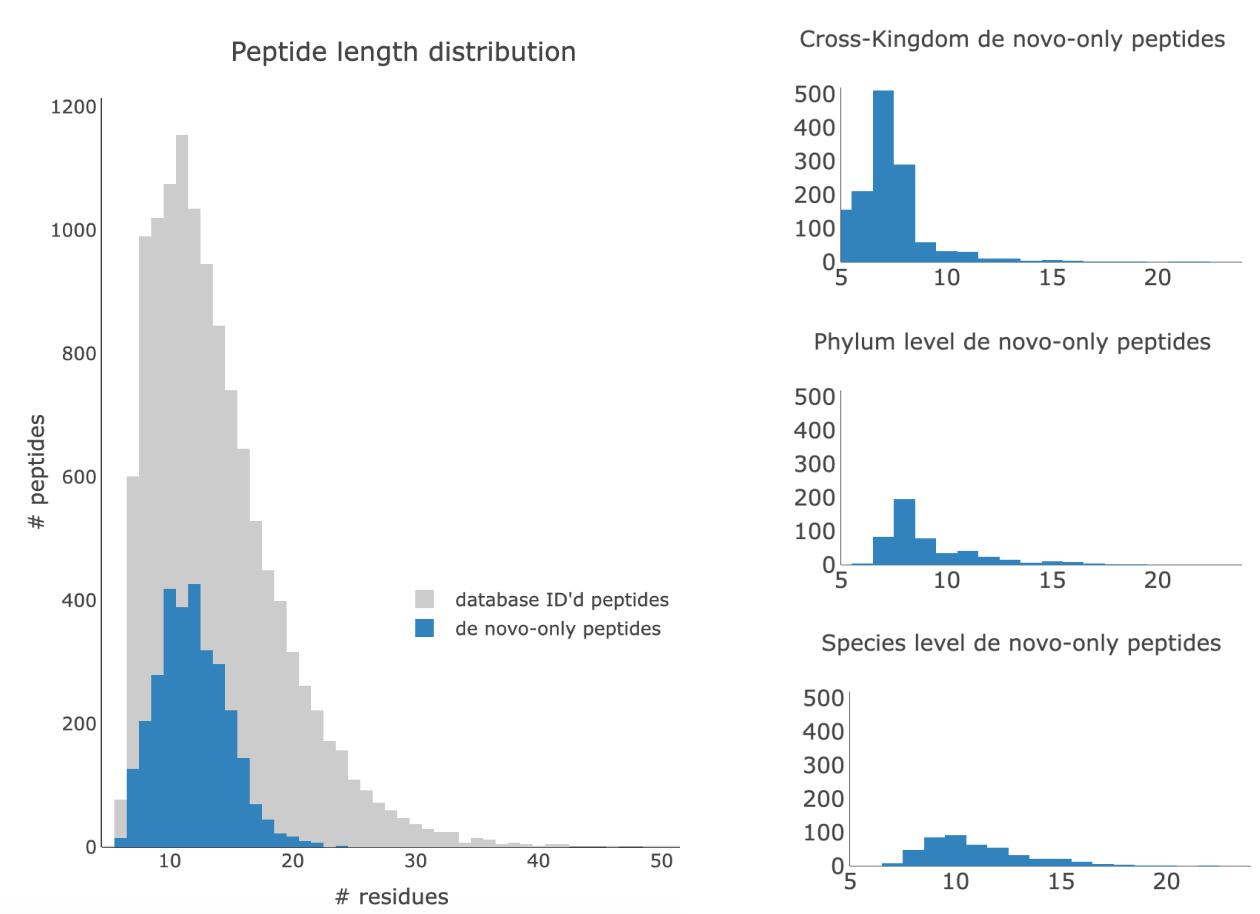
\includegraphics[width=\linewidth]{fig1-denovo.jpg}
	\caption{Histograms showing a) overlaid distributions of sequenced peptide lengths (number of amino acid residues) for database search-identified (grey) and \textit{de novo}-only peptides (blue) of cultured \textit{Prochlorococcus marinus} MED4 protein LC-MS/MS dataset. Of 12,160 database peptides, the mean length was 13.8 residues; of 3,019 \textit{de novo} peptides, the mean length was 10.9 amino acids. Distributions of \textit{de novo}-only peptide lengths for individual taxonomic rankings are shown for b) cross-kingdom, c) phylum, and d) species.}
	\label{fig:de-novo-hists}
\end{figure}

In this benchmark study of the \textit{P. marinus} HRMS spectral dataset, I performed \textit{de novo} peptide sequencing with a commercially available algorithm, Peaks \cite{ma_peaks:_2003}, and database searching, aligning and comparing the two resulting groups of peptides on several criteria: coverage of the known \textit{Prochlororoccus} proteome, degree and types of mass modification, length (number of amino acids), and taxonomic specificity (the degree to which a certain peptide is identifying of and unique to one organism's protein sequence or many across different taxa.)

In terms of proteome coverage, \textit{de novo} sequencing did as well as expected: 28\% identification rate of the total predicted proteins, compared with 67\% for traditional database searching. However, the \textit{de novo} algorithm did find peptides unidentified through database searching that boosted the overall protein identification rate by 6\%. The \textit{de novo} peptides were, on average, almost 3 residues shorter than the average of the database-identified peptides [Figure \ref{fig:de-novo-hists}]. Peptide length is an important metric in an metaproteomic and peptidomic context because with increased amino acid space, peptide sequences have more potential to be specific to a particular parent protein. Given the limitations of \textit{de novo} sequencing, we expect the lengths of confident \textit{de novo} peptides to be shorter than those identified by database searching. 

To establish the specificity of \textit{de novo}-only sequences (\textit{de novo} sequences that did not align with database-ID'd peptides), I interrogated their sequences against the UniProt Knowledgebase (UniProtKB) protein database using Unipept, a tool designed for tryptic peptide sorting and identification. Unipept uses a lowest common ancestor (LCA) approach to match peptides to as low a resolved taxonomic identification level as is possible given the input sequence. I found that many \textit{de novo}-only peptides are taxonomically specific, with 17\% specific to at least the phylum Cyanobacteria, and 15\% specific to the species level [Figure \ref{fig:de-novo-hists}]. In contrast, of the database-identified peptides; 51\% of peptides matched to the species level. Overall, this comparison showed that the \textit{de novo}-only peptides sequenced from the \textit{Prochlorococcus} culture data are not as specific to their organismal source to those sequenced by traditional database searching, but still have potential to identify individual organisms in a mixed community.  It is important to note that the \textit{de novo}-only non-specific peptides, while not taxon-identifying, nevertheless represent valuable information, especially if one is less concerned about organismal source and wishes to evaluate sequence similarity with respect to preservation and degradation.  

I searched for 30 different mass modifications, and the seven most commonly observed in this dataset were carbamidomethylation (on cysteine), oxidation (on methionine), acetylation, formylation, deamidation (on asparagine and glutamine), dehydration and phosphorylation. Since carbamidomethylation is performed during experimental peptide preparation and set during both database and \textit{de novo} searches, we expect no difference in levels of this modification been the peptide pools. Indeed, no significant difference in carbamidomethylation is observed between database and \textit{de novo}-only peptides. However, in the case of every other modification we searched for, the \textit{de novo}-only peptides are more modified - by up to 10\% more in the case of acetylation and to lesser extents for oxidation, formylation, deamidation, dehydration, and phosphorylation. 

Thus, the culture study shows that while the results of \textit{de novo} searches are not as comprehensive in coverage as the database approach, \textit{de novo} sequencing does complement the database search by a) identifying peptides that wouldn’t otherwise have been discovered, b) identifying peptides that have been post-translationally modified, and c) providing output of non-specific peptides for further evaluation. 

\subsubsection{Preliminary environmental application: the eastern tropical North Pacific}

The exciting application of \textit{de novo} peptide sequencing is to uncharacterized systems, exemplified by the challenges to marine metaproteomic and peptidomic study. In this preliminary study as part of my M.S. work, I evaluated six POM samples from the eastern tropical North Pacific (ETNP) oxygen deficient zone (ODZ) collected in January, 2017 onboard the \textit{R/V Sikuliaq}. POM samples were collected with large volume \textit{in situ} pumps that filtered between 300 and 1000 L of seawater onto 0.3 $\mu$m membranes, which is presumed to include both free-living microbes as well as small suspended detrital organic matter. These samples are hence called suspended particles. Sinking particles were collected with free-drifting, unpoisoned sediment net traps with deployments lasting between 24 and 96 hours. 

I applied the \textit{de novo}-assisted approach to this small ETNP POM sample set, finding that \textit{de novo}-identified peptides included matches to proteins from unanticipated taxa, including many from the fungal subkingdom Dikarya. I also sequenced peptides from the autotrophic phylum \textit{Cyanobacteria} in particles at 1000 m depth, indicating transfer of autotrophic C and N from these surface microbes. Some of these peptides were missed by the database-driven approach, likely because they are in the process of being degraded as they sink to the interior of the ocean – indeed, \textit{de novo}-identified peptides at depth contain more mass modifications relative to those at epipelagic base, including deamidation and oxidation. Deamidation has been hypothesized as a source of ammonium supporting anammox in this region \cite{van_mooy_impact_2002}, suggesting that the \textit{de novo} tool provides a molecular-level view into the processes fueling chemoautotrophy.

\subsubsection*{Progress}

Both the benchmark \textit{Prochlorococcus} peptide analysis and ETNP POM study, was submitted to \textit{Limnology and Oceanography} in January, 2020 and is currently under review. The \textit{de novo}-assisted peptide sequencing approach is used in Chapter 2, 3, and 4. 

\subsection{Chapter 2: Tracking protein breakdown in a controlled algae degradation}

\textit{De novo}-assisted peptide sequencing was used to investigate changes in peptide quality over the course of a semi-controlled degradation of a diatom culture in natural seawater. Proteins were extracted and trypsin-digested from a bloom-and-bust simulation sampled at multiple timepoints. This builds upon both laboratory \cite{nunn_path_2010} and environmental investigations \cite{moore_identifying_2012} of protein breakdown. The latter example, from 2012, in which Moore and colleagues tracked diatom proteins from surface to early sediments in the Bering Sea, highlights how far metaproteomic instrumental and algorithmic tools have advanced in a short time: they identified 4 \textit{Thalassiosira pseudonana} proteins in the surface and just 1 into early sediments through traditional database searching. We are now able to sequence and identify hundreds of algal proteins in each timepoint in this degradation dataset. 

\bigskip

\textbf{Question 2.1} How does the peptide pool of the phytoplankton change through degradation?


Recent work by Abdulla and colleagues showed an accumulation in anoxic sediment pore water of what seem to be deaminated peptides (shown through FTIRMS, and not proteomic sequencing, \cite{abdulla_accumulation_2018})I hypothesized that sequenced peptides would become: 

\renewcommand{\labelenumi}{\alph{enumi}}
\begin{enumerate}
	\item[a)] shorter in length
	\item[b)] more non-tryptic in character (lower tryptic:non-tryptic ratio)
	\item[c)] more modified, particularly with more oxidation and deamidation
	\item[d)] closer to DI index relative amino acid ratios
	\item[e)] increasingly from membrane-associated proteins
\end{enumerate}

\subsubsection{Experimental design}

A culture of marine diatom \textit{Thalassiosira weissflogii} brought to approximately 106 cells/mL, concentrated, rendered non-viable by freezing at  -80 C, then homogenized. This frozen concentrate was thawed, resuspended to 2 g/L (dry weight) in 1 $ \mu $m filtered, UV-sterilized surface seawater collected from the Gulf of Maine (GoM). Algal cells in suspension were confirmed intact by microscopy. Unsterilized, 1 $ \mu $m filtered filtered GoM seawater used to induce bacterial decomposition of algal material: 1  mL added to 1 5L of seawater. The algal suspension was covered in black plastic and left undisturbed in the dark at 19.5 C, monitored daily and sampled for chemical analyses at days 0, 2, 5, and 12. Algal cell counts were estimated by chlorophyll autofluorescence and the abundance of bacterial cells indicated by SYBRGreen staining. 


\subsubsection{Peptide evolution over degradation of \textit{T. weissflogii culture}}

To make a protein search database, I extracted \textit{T. weissflogii} transcript sequences from the Marine Microbial Eukaryote Transcriptome Sequencing Project (MMETSP) \cite{keeling_marine_2014} and GoM metagenomic sequences from the Global Ocean Sampling (GOS) data product \cite{yooseph_sorcerer_2007}.
 
 Application of \textit{de novo}-assisted database searching reveals changes in peptide composition over degradation by a natural microbial community. Both tryptic and non-tryptic peptides sequenced from late-stage degradation material are relatively enriched amounts of glycine, serine, and threonine and depleted phenylalanine, glutamic acid, tyrosine, and leucine. While similar observations of relative amino acid abundance patterns have been made for organic matter degradation on a bulk level by looking at total hydrolyzable amino acids \cite{dauwe_linking_1999}, this is the first observation that the enzyme-hydrolyzable peptide pool influences this pattern. Because \textit{de novo} sequencing is not reliant on a protein database, we are also able to identify proteins or protein fragments from organisms unexpected in the sample, particularly useful later stages of the time series degradation sequence. The chemical and phylogenetic specificity contained in peptide sequences enables the tracking of protein degradation along a presumed early diagenetic sequence, opening the door for more insights into the origin, evolution and fate of proteinaceous materials under varying ocean conditions.

\subsubsection{Evolution of peptide mass modifications}

Comparison of total modification distribution to DI papers. Serine abundance. Future directions of this kind of work?

\subsubsection*{Progress}



\subsection{Chapter 3: High-resolution marine flux measurements and \textit{in situ} respiration rate determinations, and metaproteomic surveys of particulate matter in the eastern tropical North Pacific oxygen deficient zone}

\subsubsection{Study site: the eastern tropical North Pacific}

Oxygen deficient zones (ODZs) naturally occur where aerobic respiration of organic matter (OM) combines with water column stabilization to form a persistent, low-oxygen layer at mid-depths. ODZs make up less than 1\% by volume of the world ocean, yet account for 30-50\% of the oceanic nitrogen loss as N\textsubscript{2} \cite{devries_marine_2013}, driving nitrogen limitation of primary productivity over vast regions of the ocean. The size of ODZs is sensitive to climate change and variability: a 1\% reduction of the ocean’s  O\textsubscript{2} content is predicted to double the size of world OMZs \cite{deutsch_climate-forced_2011}. Critically, climate models predict an approximate 5\% decrease to the ocean’s O\textsubscript{2} reservoir within this century \cite{bopp_multiple_2013}. 

The exciting application of \textit{de novo} peptide sequencing is to uncharacterized systems, perfectly exemplified by the challenges to marine metaproteomic and peptidomic study. The eastern tropical North Pacific (ETNP) is home to the Earth’s largest marine oxygen deficient zone (ODZ), accounting for approximately 41\% of global marine anoxic waters \cite{paulmier_oxygen_2009}. Numerous studies have documented an ‘enhanced’ flux through ODZs, implying that a high fraction of the surface-derived particulate organic carbon sinks to the deep ocean \cite{devol_role_2001, van_mooy_impact_2002, keil_multiproxy_2016}. However, there remains much uncertainty about the mechanism(s) explaining these observations. In the ODZ, shifts in zooplankton behavior \cite{keil_multiproxy_2016} and \textit{in situ} production from anammox \cite{ganesh_single_2018} or deep photoautotrophy by \textit{Prochlorococcus} populations within the anoxic secondary chlorophyll maximum (Fuchsman et al. 2019) likely have roles in an enhanced flux. These POM fluxes are important in controlling N\textsubscript{2} loss from denitrification and anammox \cite{fuchsman_cyanobacteria_2019} and likely the makeup of POM controls the relative contribution of those processes \cite{babbin_organic_2014}. Since proteinaceous matter comprises the single largest identifiable component of the sinking flux in the tropical eastern Pacific \cite{wakeham_molecular_1997}, evaluating its processing using the de novo-assisted approach might provide insights POM dynamics and carbon and nitrogen flow in within this ODZ. 

\bigskip

\begin{figure}
	\includegraphics[width=\linewidth]{pomz-sed-trap-sta.jpg}
	\caption{The eastern tropical North Pacific oxygen deficient zone (ETNP ODZ), shown here as O\textsubscript{2} concentration at 200 m from World Ocean Atlas data, 1955-2013. Time series sediment trapping stations (P1, P2, and P3) for the three POMZ expeditions are shown with expedition timings.}
	\label{fig:etnp map}
\end{figure}

My goal is to combine peptide-level molecular determinations with flux and metabolic rate measurements to learn about the microbial actors, their fuel, and quantitatively, the biogeochemical implications of their lifestyles. This can be described in three primary questions:

\bigskip

\textbf{Question 3.1} How variable are OM flux profiles across seasons and from on to offshore? Is there a shift in microbial community structure and OM processing when these profiles look different?

\bigskip

\textbf{Question 3.2} Are there patterns in peptide and protein degradation in sinking and suspended POM, with depth and between on- and offshore stations?

\bigskip

\textbf{Question 3.3} How variable are OM flux profiles across seasons and from on to offshore? Is there a shift in microbial community structure and OM processing with  when these profiles look different?



\subsubsection{Field Work and Preliminary Observations}

Describe 3 cruises here. Describe sediment traps, briefly, and McLane pumps. Figure \ref{fig:etnp map} the locations and timings of ETNP station sediment trap sampling. 


\subsubsection{Flux of suspended and sinking POM from 2017-2019}

This highly collaborative work addresses \textbf{Question 3.1}. The Keil group has deployed sediment trap-incubator systems and large volume \textit{in situ} pumps (McLane) on three recent research cruises to the ETNP between January, 2017 and October, 2019 (see Figure \ref{fig:etnp map}).

\bigskip

Fluxes from 2017-2018 here. Make an R version from talk Excel fig. 

\subsubsection{Metapeptidomic and metaproteomic signatures of POM through the ODZ}

Table of run proteomics samples and extracted proteomics samples.

For a functional analysis of OM processing, I'll use the peptide-based tool Unipept \cite{uniprot_consortium_uniprot:_2018} to identify peptides indicative of certain metabolic processes based on gene ontologies, or GO terms. Unipept uses peptide spectral counts to generate semi-quantitative BLAST-like sequence alignment against a manually annotated and reviewed section of the UniProtKB database.

\begin{figure}
	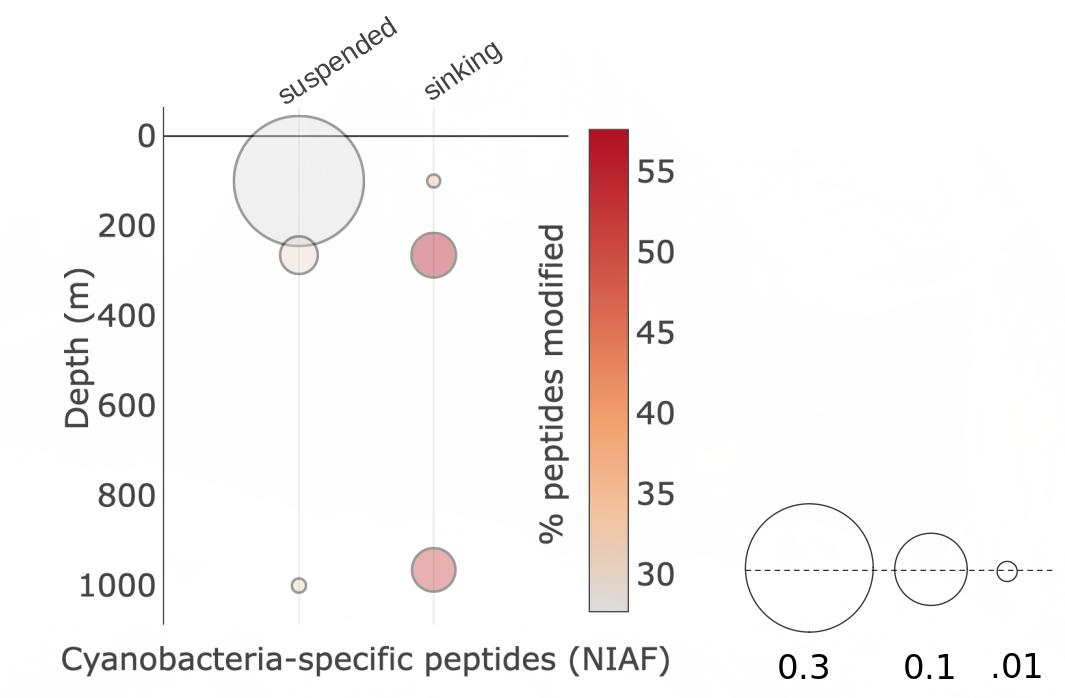
\includegraphics[width=\linewidth]{etnp2017-cyano-mods.jpg}
	\caption{Cyanobacteria-specific peptides sequenced from suspended and sinking POM from offshore Station P2, ETNP January 2017 with sampling depth. Bubble sizes represent peptide abundances scaled by the normalized ion abundance factor (NIAF) of the MS1 parent ion spectral counts. Color scale represents the percentage of peptides in each samples with mass modifications.}
	\label{fig:cyanomods}
\end{figure}

Figure \ref{fig:cyanomods} shows the relative numbers of peptides sequenced and identified as exclusively belonging to the phylum \textit{Cyanobacteria} in suspended and sinking particles from offshore Station P2 in the ETNP, January 2017. Color scale indicates the percentage of peptides in each sample that have mass modifications as described in Section 1.2.

\subsubsection{Metabolic rate calculations from \textit{in situ} incubation-sediment traps}

2017 and 2018 rates here. 

\subsubsection*{Progress}

\subsection{Chapter 4: Organic matter exchange in the Lower Amazon River}

\subsubsection{The Lower Amazon River-to-Ocean Continuum}

Water is a major vector that moves biogeochemical constituents through Earth's reservoirs and across the continuum of the atmosphere, biota, soils, inland waters, oceans, and sediments \cite{Cole2007Plumbing}. Biological and physical mechanisms like weathering, production, respiration, as well as human land use serve to transform organic carbon-containing molecules along their journey through these systems. The classically conceived role of rivers in this transport is that they simply export OM to the oceans and that once there, long-term preservation of terrestrially-derived OM occurs largely along continental margins. However, in recent decades rivers have come to be seen not simply as transitory pipes, but as themselves transformers and regulators that adjust the carbon cycle of not only their watersheds but also of the marine receiving waters. This paradigm shift is a result of the discovery that rivers and other inland waters outgas immense quantities of CO\textsubscript{2} and CH\textsubscript{4} to the atmosphere \cite{butman_significant_2011, richey_outgassing_2002}. 

Globally, it's estimated that inland waters process, transport, and bury 2.7 Pg C y\textsuperscript{-1} \cite{battin_boundless_2009, tranvik_lakes_2009}. As this figure nearly equals current estimates of the terrestrial sink for anthropogenic carbon (2.8 Pg C y\textsuperscript{-1}) \cite{canadell_contributions_2007}, carbon cycling in rivers then relocates and/or mitigates terrestrial sequestration of human forcing. But estimating these riverine carbon fluxes is logistically difficult, and depending on their actual magnitude, the global terrestrial CO\textsubscript{2} sink may prove to be smaller than currently estimated because rivers may mobilize and remineralize a significant component of the OM pool that is considered sequestered in soils. This poses two primary questions – \textbf{what are the geographic distributions and magnitude of aquatic CO\textsubscript{2} outgassing, and what are the dynamics that drive this outgassing?} 

The high levels of CO\textsubscript{2} supersaturation that drive gas evasion from large rivers are thought to be largely produced through \textit{in situ} respiration by heterotrophic microbes. These communities utilize OM that is fixed on land and then flushed into rivers as a substrate \cite{mayorga_young_2005, ward_degradation_2013, ward_reactivity_2016}. However, there is little knowledge of what terrestrial OM compounds actually fuel this respiration or the range of their turnover rates. Work done in marine systems and small streams has propagated an assumption that lignin and cellulose, the two major classes of macromolecles in terrestrial OM, are generally refractory in all aquatic systems \cite{hedges_fluxes_1988, gough_terrestrial_1993, opsahl_distribution_1997}. However, recent work in the lower Amazon basin have shown that lignins do in fact contribute to heterotrophic respiration in the main stem of the river \cite{ward_degradation_2013}. In particular, rotating incubation systems that better simulate the flow conditions of the river have been important in deciphering the source of highly reactive materials \cite{ward_marine_2018}. This is critical to understanding the remineralization potential of specific OM types and to elucidating the underlying mechanisms controlling their fate. 

Such developments have made significant headway towards achieving the ultimate goal: calculating of the overall carbon balance of a basin and making predictions of future change. Outstanding unknowns to achieving this goal are: evaluating the types of OM that are degraded in the river, their sources, the microorganisms and consortia that degrade the fixed carbon, and the metabolic pathways (aerobic, anaerobic) that lead to the large outgassing of CO\textsubscript{2} and CH\textsubscript{4}. A large team of scientists from Brazil and the U.S. led by Dr. Jeff Richey is funded to address these issues in the world's largest river system, the Amazon, using a combination of organic geochemical and molecular biological tools. My role in this collaboration is 1) providing a proteomic window into the microbial community processing of OM as it changes along the continuum and with hydologic conditions, and 2) characterizing the proteinaceous component of this OM along the same gradients. The primary research question I will address are:

\bigskip

\textbf{Question 4.1} What is the microbial community composition and functioning of the lower river-to-ocean transition, and what are the OM degradation pathways fueling the observed CO\textsubscript{2} exchange? Do these shift with different hydrologic regimes (high vs low water)?

\bigskip

\textbf{Question 4.2} How do different components of terrestrial OM (proteins, lignins, black carbon), cycling in the river-to-ocean continuum across the different flow regimes of the year? 

\bigskip

As detailed below, I will address \textbf{Question 4.1} using a combination of \textit{de novo}-proteomics, underway hydrologic and gas flux measurements, and metatransciptomic analyses from previous \cite{doherty_bacterial_2017, satinsky_amazon_2014} and current collaborators. I'll address \textbf{Question 4.2} using the aforementioned datasets and collaborators' geochemical measurements of lignin, amino acids, and POM/DOM characterization. 

\subsubsection{Field Work and Preliminary Observations}

\begin{figure}
	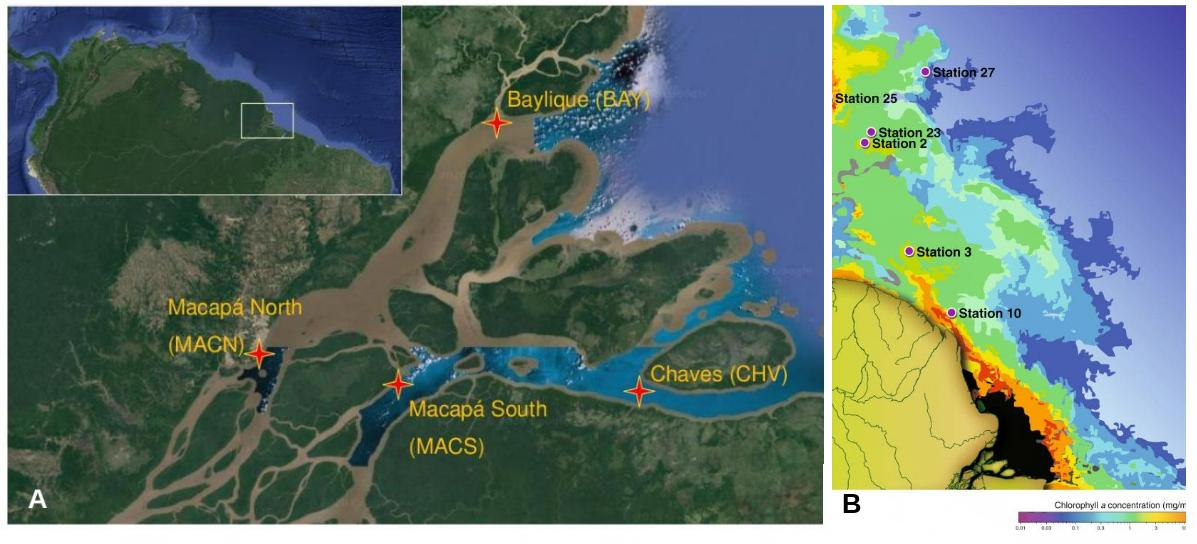
\includegraphics[width=\linewidth]{amazon-sta-map.jpg}
	\caption{Lower Amazon sampling stations, April 2019. }
	\label{fig:amazon-stations}
\end{figure}

I've participated in one lower Amazon expedition (April, 2019) and had additional samples collected in November, 2019. Currently I have large suite of metaproteomics samples (approximately 200 with replicates) from 4 stations of the lower Amazon reach (Figure \ref{fig:amazon-stations}), spanning high- and low- water regimes of the hydrograph, as well as across tidal cycles. I plan to participate in, or get samples from, a future expedition on a boat capable of reaching further into the plume (timing TBA, given current events). This will connect sampling from earlier Richey-led Amazon projects, TROCAS I (upriver from Macap\'{a}) and ROCA (into the Atlantic plume).

\bigskip

Map of TROCAS I and ROCA stations

\bigskip

\textbf{I hypothesize that community structural and functional shifts will co-occur with changes in DOM composition.} In particular, I expect that the abundance of proteins related to specific functions (e.g. lignin degradation, primary production, and nutrient cycling) will be closely related to changes in DOM molecular formulae throughout tidal cycles, incubations, and along the study domain. Protein abundance will rapidly respond to changing conditions, revealing microbial stress signals and processes that are too dynamic/rapid to capture through traditional genomics. I anticipate microbial community shifts to be structured by hydrographic and tidal conditions, as has been found in Arctic rivers to the point of using genes as an accurate predictor river discharge (‘genohydrography’, \cite{good_predicting_2018}). Several other studies have established links between river flow rates and community composition \cite{crump_synchrony_2005}, including out in the Amazon plume \cite{doherty_bacterial_2017}. 
There is precedent for anticipating that two scenarios: first, where a microbial community shifts in composition with changing OM. For example, in a study of an Arctic fjord, Paulsen and colleagues identified specific taxa that were associated with degradation of fluorescent DOM (FDOM) \cite{paulsen_biological_2019}. In a second scenario, the functioning of the community the the main response to OM, as shown in recent metaproteomic work by Mikan and colleagues with similar aims in to this project in the Chuchki Sea. They showed a shift in functional response to OM shifts in shipboard incubations simulating a phytoplankton bloom, with some slight change in the heterotrophic community makeup \cite{mikan_metaproteomics_2020}.

Figure \ref{fig:amazon-stations} shows the 4 proteomics/DOM/incubation stations sampled in April, 2019 at rising water on the \textit{B/M Mirage}. All four stations were also sampled for full cross channel ADCP current velocity profiles over tidal cycles, total suspended sediments, nutrients, total C and N, and gas exchange. 

\bigskip


\subsubsection{Degradation tracking incubation experiment}

While my goal is to enlarge the geographical lens of research in this section of the river and make connection to the DOM pools, I'm also interested in timescales of bacterial DOM transformations and the resulting reactivity of processed material. For this reason, I conducted incubations in river condition-mimicking rotating chambers in triplicate \cite{ward_marine_2018}. 

\subsubsection*{Progress}


\begin{enumerate}
	\item[1.] Extracted protein from the April 2019 water and incubation samples in duplicate in the lab at UW in preparation for LC-HRMS when the UW Proteomics Resource Center (and campus) is open again. Protein extraction concentrations as determined by a Lowry assay show sufficient protein for analysis. 
	\item[2.] Constructed a search database from previous upriver and plume expeditions' metagenomic and metatransciptomic publications \cite{satinsky_amazon_2014, doherty_bacterial_2017, satinsky_metagenomic_2015, ghai_metagenomics_2011}.
\end{enumerate}


\newpage

\section{Timeline of research}

Combined M.S./Ph.D. from September 2015 - September 2021 (6 years):

\bigskip

\textbf{Winter 2020}
\begin{itemize}
	\item Co-instruct Ocean 295: Chemistry of Marine Organic Carbon
	\item Presentations: Ocean Sciences Meeting
	\item Lab work: Chp 4 Amazon proteomics
	\item Writing: Chp 2 Algae rot
	\item Funding: NSF GRFP
\end{itemize}

\textbf{Spring 2020}
\begin{itemize}
	\item Data analysis: Chp 3 ETNP metapeptidomics
	\item Lab work: Chp 4 Amazon proteomics
	\item Funding: NSF GRFP
	\item Apply for DOE student grant
\end{itemize}

\textbf{Summer 2020}
\begin{itemize}
	\item Outreach: Ocean Intern (3-4 weeks)
	\item Waterhackweek (August 31-Sept 6th)
	\item Writing: Chp 3 
	\item Funding: NSF GRFP
\end{itemize}

\textbf{Autumn 2020}

\begin{itemize}
	\item Funding: NSF TROCAS II
\end{itemize}

\textbf{Winter 2021}

\begin{itemize}
	\item Funding: NSF TROCAS II
\end{itemize}

\textbf{Spring 2021} 

\begin{itemize}
	\item Funding: NSF TROCAS II
\end{itemize}

\textbf{Summer 2021} 

\begin{itemize}
	\item Funding: NSF TROCAS II
\end{itemize}

\textbf{Autumn 2021} 

\begin{itemize}
	\item Funding: NSF TROCAS II
\end{itemize}



\newpage

\section{References}

\printbibliography[heading=none]

\end{document}
